\documentclass{article}
\usepackage[UTF8]{ctex}
\usepackage{pythonhighlight}
\usepackage{listings}
\lstset{
    basicstyle          =   \tt,          % 基本代码风格
    identifierstyle=\color{brown!80!black},
    keywordstyle        =   \color{purple}\bfseries,          % 关键字风格
    commentstyle        =   \rmfamily\itshape,  % 注释的风格,斜体
    stringstyle         =   \ttfamily,  % 字符串风格
    flexiblecolumns,                % 别问为什么,加上这个
    numbers             =   left,   % 行号的位置在左边
    showspaces          =   false,  % 是否显示空格,显示了有点乱,所以不现实了
    numberstyle         =   \zihao{-5}\ttfamily,    % 行号的样式,小五号,tt等宽字体
    showstringspaces    =   false,
    captionpos          =   t,      % 这段代码的名字所呈现的位置,t指的是top上面
    frame               =   lrtb,   % 显示边框
    backgroundcolor=\color[RGB]{245,245,244},
}
% Language setting
% Replace `english' with e.g. `spanish' to change the document language
\usepackage[english]{babel}
\usepackage{float}
% Set page size and margins
% Replace `letterpaper' with `a4paper' for UK/EU standard size
\usepackage[letterpaper,top=2cm,bottom=2cm,left=3cm,right=3cm,marginparwidth=1.75cm]{geometry}

% Useful packages
\usepackage{amsmath}
\usepackage{graphicx}
\usepackage[colorlinks=true, allcolors=blue]{hyperref}

% 标题、日期、作者信息在前面
\title{数据库实验报告1}
\author{雷远航 / 3210105807}
\date{2023.3.11}


\begin{document}

%\tableofcontents
% 可用于目录的生成


\maketitle


\begin{abstract}
    实验一: DBMS的安装和使用
\end{abstract}






\section{实验目的}

\subsection*{- 通过安装某个数据库管理系统,初步了解 DBMS 的运行环境。}


\subsection*{- 了解 DBMS 交互界面、图形界面和系统管理工具的使用。}




\subsection*{- 搭建实验平台。}


\section{实验平台}
\subsection*{- 操作系统:MacOS}
\subsection*{- 数据库管理系统:MySQL}

\section{实验内容和要求}

\subsection{安装 MySQL }

在 MacOS 的终端中安装命令行版本的 MySQL.

输入指令:`mysql -uroot -p` 即可以进入. 

\begin{figure}[H]
	\centering
	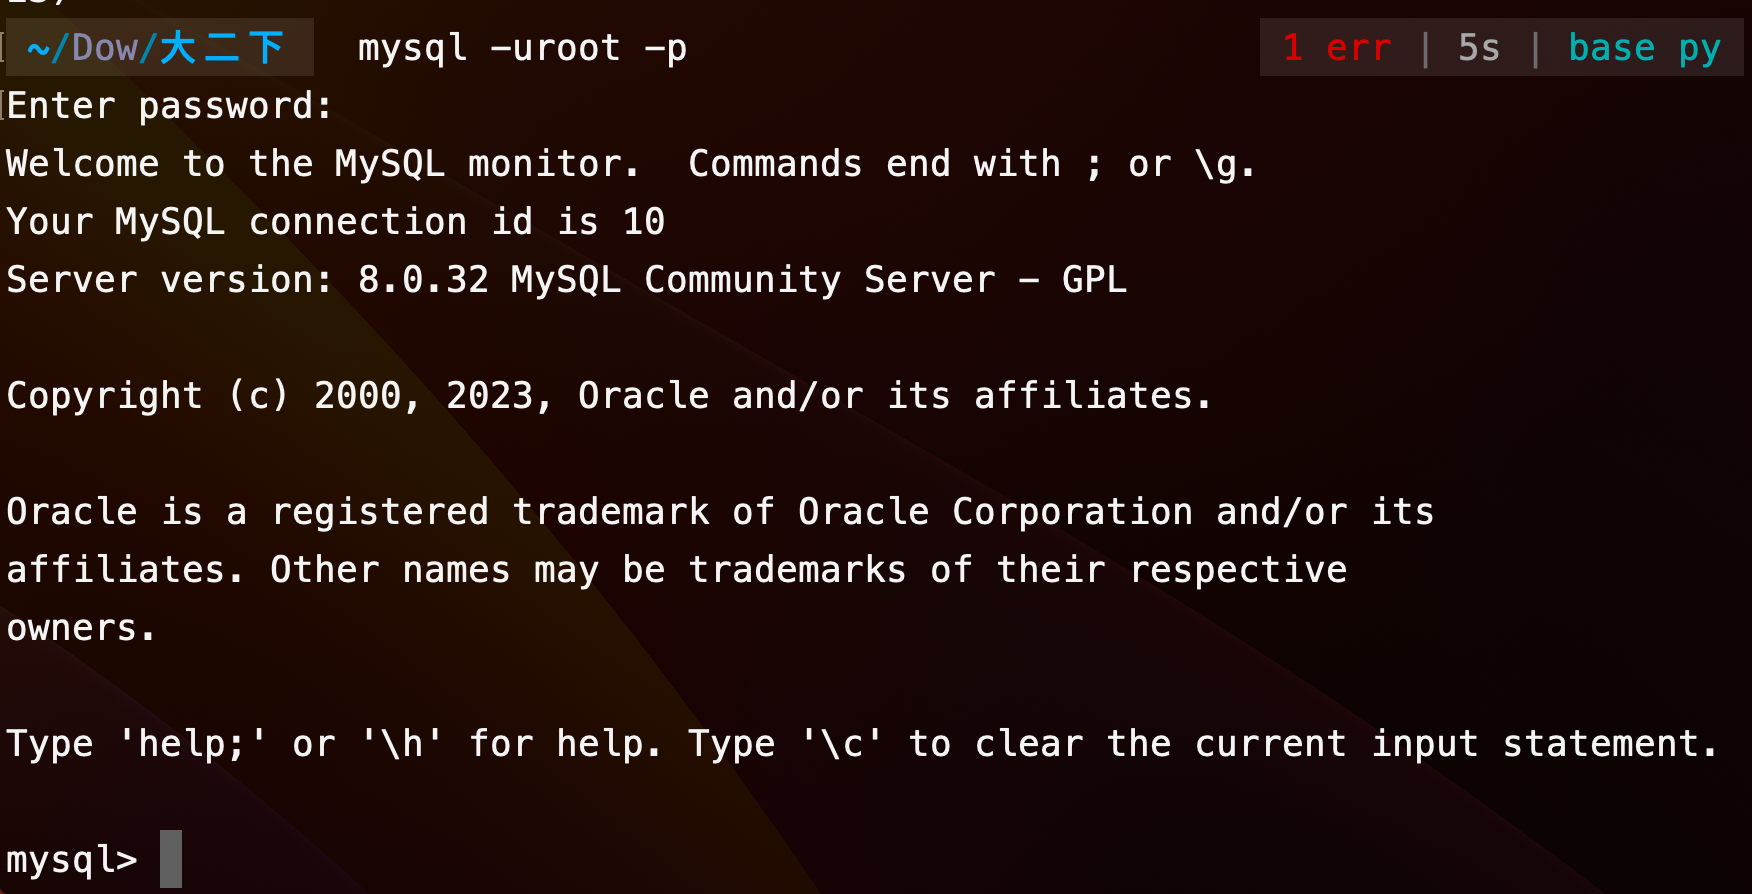
\includegraphics[width=0.7\textwidth]{lab1/1.png}
	
	\end{figure}


我们可以在 MySQL 中创建一个新用户并且为其设置一个密码。
    \begin{figure}[H]
        \centering
        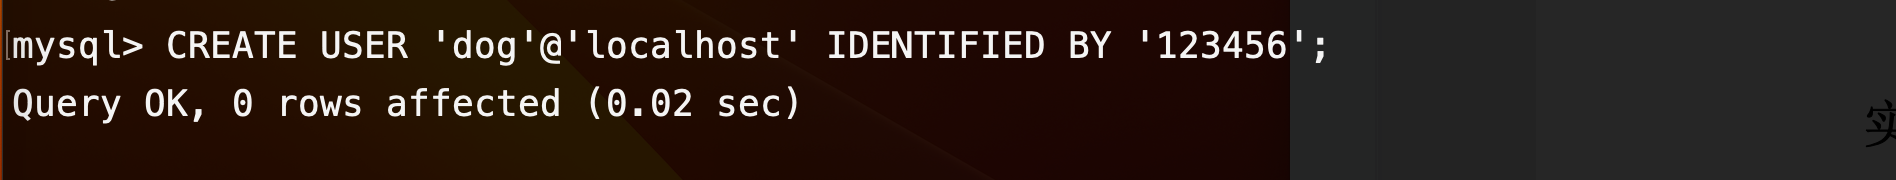
\includegraphics[width=0.7\textwidth]{lab1/5.png}
        \end{figure}


\subsection{创建数据库和表}

创建一个新的数据库: db02

在其中创建一张表: aaa 

过程的截图如下。

\begin{figure}[H]
    \centering
    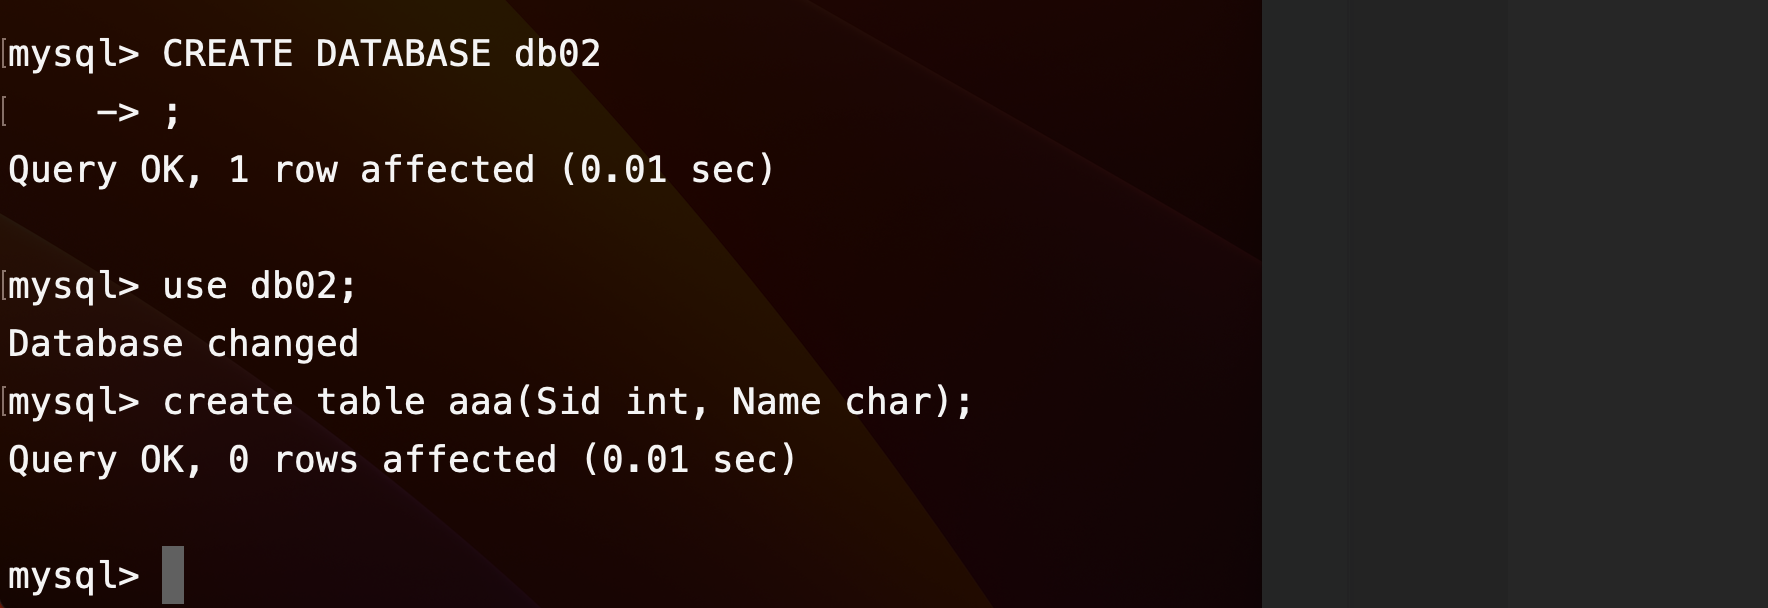
\includegraphics[width=0.7\textwidth]{lab1/3.png}
    \end{figure}


\subsection{查询语句执行}

执行 SQL 语句:`select * from aaa` 对表进行查询。

\begin{figure}[H]
    \centering
    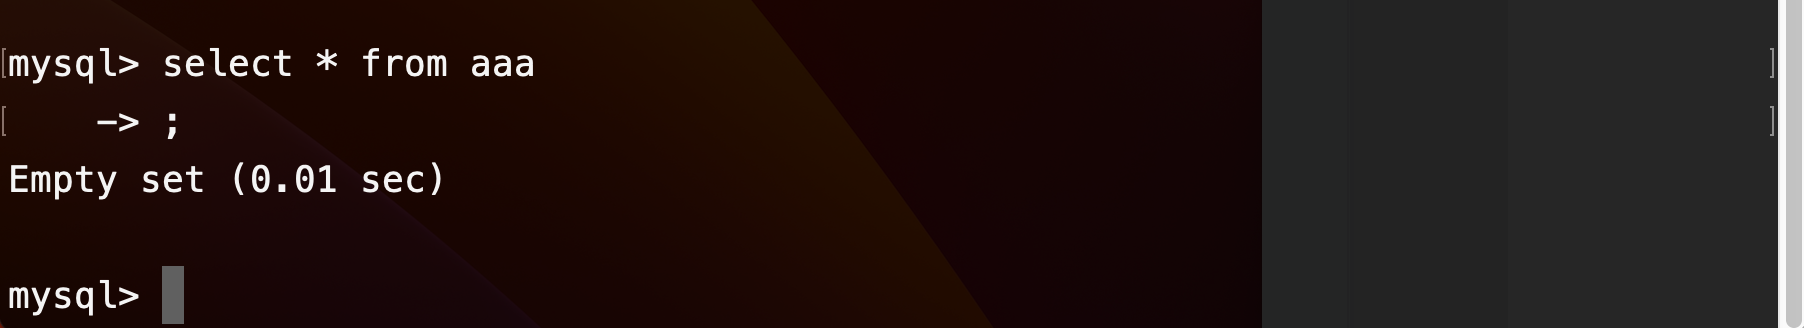
\includegraphics[width=0.7\textwidth]{lab1/4.png}
    \end{figure}

\end{document}